\documentclass{beamer}

\usepackage{amsmath}
\usepackage{amssymb}
\usepackage{graphicx}

\mode<presentation>
{
  \usetheme{Warsaw}
  % or ...

  \setbeamercovered{transparent}
  % or whatever (possibly just delete it)
}


\usepackage[english]{babel}
% or whatever

\usepackage[latin1]{inputenc}
% or whatever

\usepackage{times}
\usepackage[T1]{fontenc}

\title{Genetic burden tests}

\begin{document}

\begin{frame}
	\frametitle{Problem}
	Given the SNPs of a gene, rank the gene according to its association to some phenotype.
	\begin{itemize}
		\item Hypothesis: there are many ways to knock-out the same gene.
		\item Idea: Pool SNPs into categories using annotation, and determine association with category.
		\item Assumes that SNPs with same annotation have roughly the same effect.
	\end{itemize}
\end{frame}

\begin{frame}
	\frametitle{Data}
	\begin{itemize}
		\item Exon SNPs.
		\item Cases and controls.
		\item SNP annotation, e.g. synonymous, frameshift etc.
	\end{itemize}
\end{frame}

\begin{frame}
	\frametitle{Notation}
	\begin{itemize}
		\item Let $n$ be the number of individuals.
		\item Let $m$ be the number of SNPs.
		\item Let $t$ be the number of SNP annotation classes.
		\item Let $s_{i,j} \in \{ 0, 1, 2 \}$ be SNP $j$ for individual $i$.
		\item Let $y_i \in \{0,1\}$ be the case/control status of individual $i$.
		\item Let $a_i \in [t]$ be the annotation of SNP $i$.
		\item Let $I_g$ be the indices of the set of SNPs in gene $g$.
	\end{itemize}
\end{frame}

\begin{frame}
	\frametitle{Idea 1}
	For each gene model severity of different annotations:
	\begin{itemize}
		\item Let $x_i^g$ be the number of minor alleles of all SNPs with annotation $i$ in gene $g$.
		%\item Let $x_i$ be the number of mutation of class $i$ in all genes.
		\item Estimate
		$$ \log \frac{p}{1-p} = \beta_0 + \beta_1^g x_1^g + ... + \beta_m^g x_m^g$$
		\item Test prediction on separate test set or test significance for $\beta_1^g = ... = \beta_m^g = 0$.
	\end{itemize}
\end{frame}

\begin{frame}
	\frametitle{Idea 1}
	In more detail:
	\begin{itemize}
		\item Let $A_i^g = \{ j \mid j \in I_g, a_j = i \}$ be the indices of the SNPs with annotation $i$ that are in gene $g$.
		\item Let $x_{i,j}^g = \sum_{k \in A_j^g} s_{i,k}$ be the number of mutations of type $j$ in individual $i$ and gene $g$.
		\item The actual regression is then
		$$ \log \frac{p_i}{1-p_i} = \beta_0 + \beta_1^g x_{i,1}^g + ... + \beta_m^g x_{i,m}^g$$
		where $p_i$ is the probability of individual $i$ to be a case.
	\end{itemize}
\end{frame}

\begin{frame}
	\frametitle{Idea 2}
	Given the SNPs of a gene, rank the gene according to its association to some phenotype.
	\begin{itemize}
		\item Idea: Count mean number of "bad" mutations for each gene, and compare between case and control population.
		\item Simpler than idea 1, no weights.
	\end{itemize}
\end{frame}

\begin{frame}
	\frametitle{Idea 2}
	\begin{itemize}
		\item Let $x_i^g = \sum_{j \in I_g} s_{i,j}$.
		\item Let $P = \{ i \in [n] \mid y_i = 1 \}$, $N = \{ i \in [n] \mid y_i = 0 \}$.
		\item Compute the mean difference $$\frac{1}{|P|}\sum_{i \in P} x_i^g - \frac{1}{|N|}\sum_{i \in N} x_i^g$$
		\item Test using t-test or similar.
	\end{itemize}
\end{frame}

\begin{frame}
	\frametitle{Idea 2}
	\begin{itemize}
		\item Can also be used with case-only, by computing expected values from general population.
		\item Alt: Use binomial to model counts.
	\end{itemize}
\end{frame}

\begin{frame}
	\frametitle{Idea 1}
	Questions:
	\begin{itemize}
		\item What do we give to the biologists?
		\item How can we make sure each SNP is encoded in the right direction?
		\item How do we handle missing data?
		\item What happens if data is sparse?
		\item What other encodings of SNPs are possible?
		\item Since we are working with counts it might be more sane to model $\log p$.
		\item Support vector machines or other machine learning?
		\item Use number of rare variants, Neale et al. 2011 plos genetics.
	\end{itemize}
\end{frame}

\begin{frame}
	\frametitle{Problem}
	\begin{figure}[htbp]
		\begin{center}
			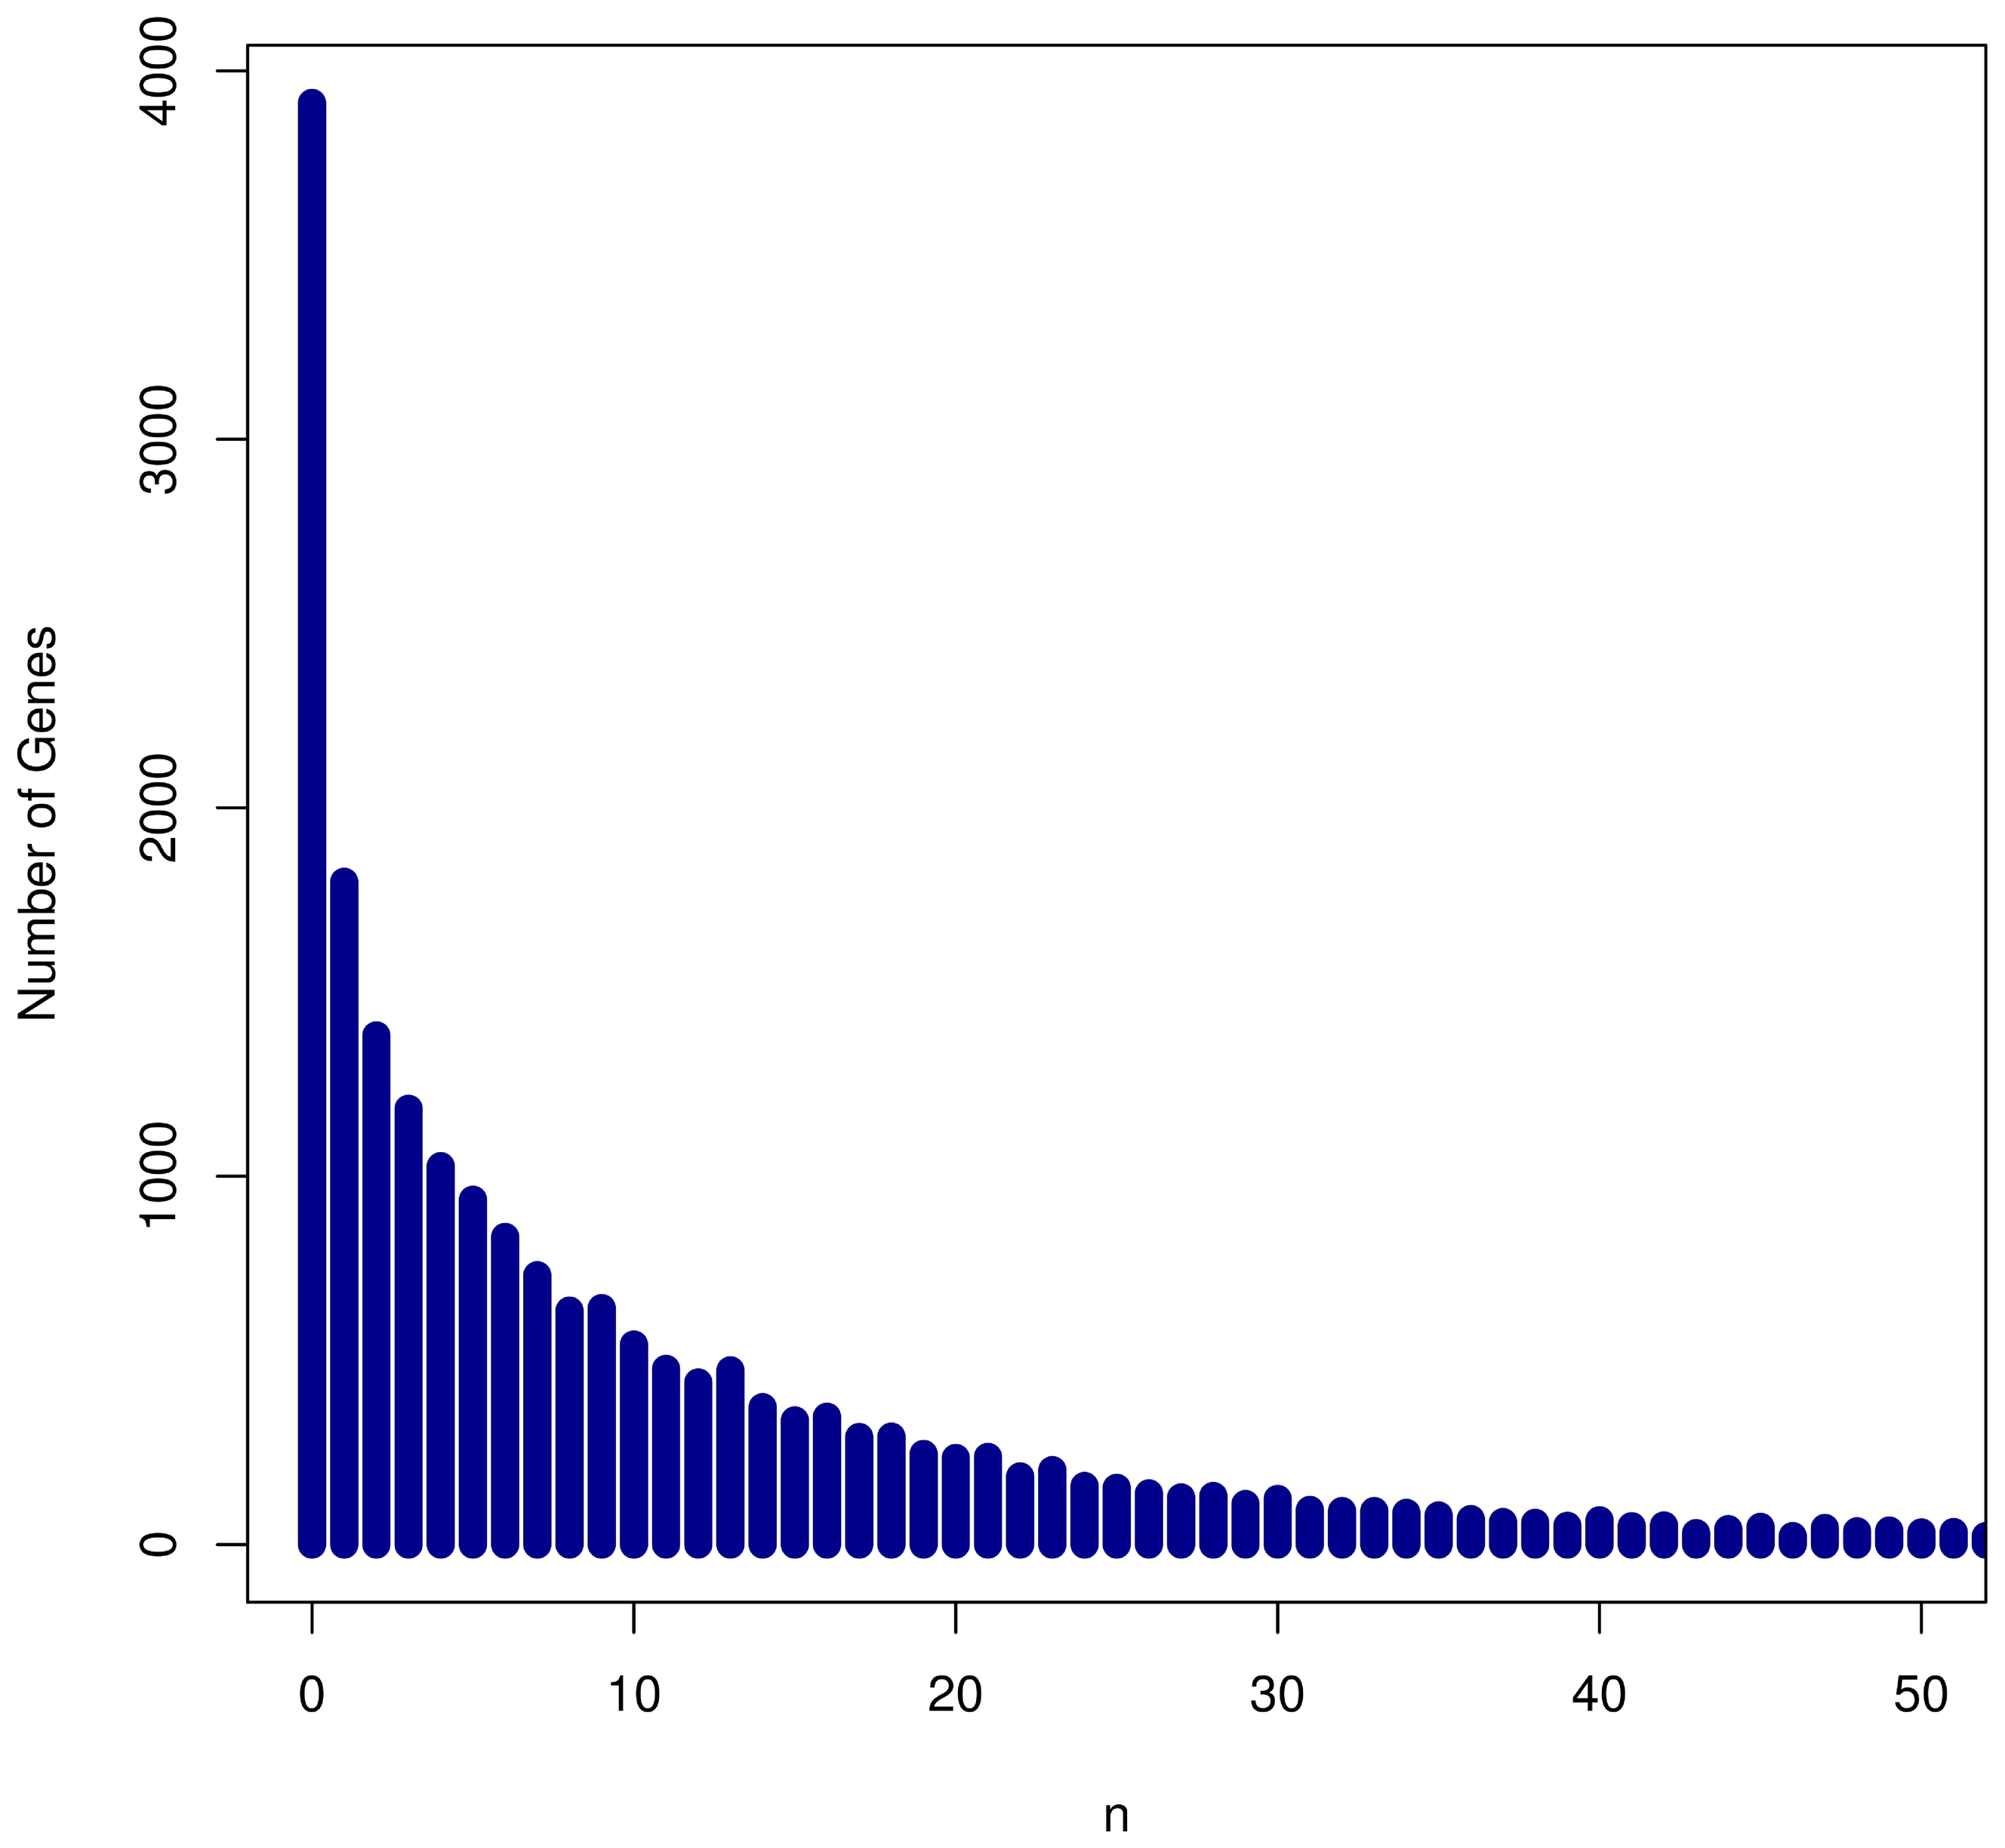
\includegraphics{snp_hist.png}
		\end{center}
	\end{figure}

\end{frame}

\end{document}